\chapter{Plano Operacional}

\section{Arranjo físico}
Para exigir o menor investimento inicial possível, a empresa exercerá suas atividades em um escritório comercial com capacidade apenas para seus quatro sócios trabalharem e um pequeno espaço para o arquivamento dos documentos que não possam ser armazenados em meio digital. Este espaço estará disposto da seguinte como visto na figura \ref{fig:escritorio} abaixo.

\begin{figure}[!h]
  \begin{center}
    \frame{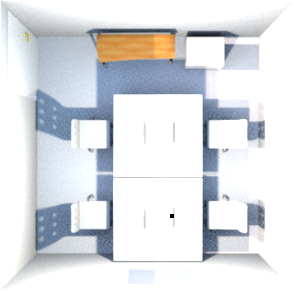
\includegraphics[width=70mm, height=60mm]{images/escritorio-frete-facil.png}}
    \caption{Vista superior da disposição do espaço de trabalho}
    \label{fig:escritorio}
  \end{center}
\end{figure}

Para tanto, o escritório será composto de 4 mesas para computador, 4 cadeiras, um arquivo e uma mesa de lado, totalizando um área útil mínima de $10m^{2}$.

\section{Capacidade produtiva}
  \subsection{Novas funcionalidades}\label{subsec:novasfuncionalidades}
  Considerando que os quatro sócios da frete fácil são programadores qualificados, com 40 horas semanais de dedicação, totalizando 160 horas de trabalho por semana.
  
  Com isto, é possível entregar pequenas melhorias\footnote{Entende-se por pequena, uma mudança de cor de fonte ou um novo ícone, por exemplo.} em questão de dois dias aproximadamente, as médias\footnote{Melhorias médias são, por exemplo, um novo campo de busca. Que não afetam a estrutura do software.} em uma semana e as grandes\footnote{Grandes melhorias afetam a estrutura do software, tendo como o exemplo o oferecimento de uma API para os clientes} podem levar mais de um mês.
  
  \subsection{Capacidade de atendimento a clientes}
  A plataforma, como será construída para funcionar na nuvem, não apresenta limitações físicas para escalar. Há apenas a limitação financeira para o crescimento da capacidade de atendimento.
  
  Em seu primeiro ano de vida, há a previsão de atender até 175 empresas de frete que realizarão até 1575 fretes (último mês do orçamento \ref{financeiro}. Caso surja uma demanda maior que esta antes do fim do primeiro ano de vida, a empresa pode recorrer ao seu caixa ou empréstimos para supri-la, visto que neste ponto a empresa já estará obtendo lucro.
  
  Considerando a sazonalidade do tipo de negócio, este estará sujeito a picos de demanda idênticos ao do comércio de varejo, visto que nossos clientes são as responsáveis por entregas decorrentes de vendas no varejo.
  
\section{Processos Operacionais}
  \subsection{Ciclo de desenvolvimento}
  O desenvolvimento de um determinado conjunto de funcionalidades na plataforma se dará seguindo o seguinte ciclo de desenvolvimento:

  \begin{enumerate}
    \item Especificação de cada funcionalidade;
    \item Estimar tempo e valor agregado à plataforma para cada funcionalidade;
    \item De acordo com as estimativas, definir um conjunto prioritário de funcionalidades que caibam dentro de um período máximo de duas semanas, que será chamado de iteração;
    \item Para cada funcionalidade definir quais tarefas devem ser completadas para a funcionalidade estar implementada;
    \item Executar as tarefas, mantendo registro durante a iteração sobre o que já foi feito, o que está sendo feito e o que ainda não foi começado.
  \end{enumerate}

  Certamente surgirão imprevistos durante este ciclo que serão absorvidos. Caso esta situação se torne frequente, as medidas a serem adotadas são:
  
  \begin{itemize}
    \item Reduzir o tempo da iteração para uma semana;
    \item Dentro da iteração já reservar certo tempo para trabalhar em imprevistos.
  \end{itemize}
  
  Por fim, este é um processo teórico já consolidado no desenvolvimento ágil, e é apenas uma base sobre a qual a empresa aprimorará o processo de acordo com suas necessidades.
  
  \subsection{Processo de aquisição de infraestrutura computacional}
  
  
  Este item, certamente será revisado assim que a plataforma estiver pronta para lançamento, quando possivelmente alguns dos serviços aqui ilustrados não serão utilizados na realidade e outros não previstos serão utilizados, além da realização de testes de carga que revelarão a real capacidade computacional necessária para esta.
  
  Porém, a para fins de ilustrar o processo, um bom ponto inicial sobre os serviços necessários, supondo toda a infraestrutura no Amazon Web Services serão:
  
  \begin{itemize}
    \item Máquinas de processamento, utilizando o serviço EC2;
    \item Máquinas para banco de dados relacional, utilizando o serviço RDS;
    \item Espaço para armazenamento de arquivos, utilizando o S3;
    \item Tráfego de dados;
  \end{itemize}
  
  A capacidade computacional estimada para estes serviços é:
  
  \begin{itemize}
    \item Uma instância EC2 \textit{small} deve suportar em torno de 30 usuários simultâneos;
    \item Uma instância média de banco de dados no RDS, deve suportar aproximadamente 100 usuários simultâneos;
    \item Cada usuário gera trafego de aproximadamente 10Mb ao mês;
  \end{itemize}
   
  Desta forma, considerando o conjunto de serviços de infraestrutura necessários para o funcionamento da plataforma e a capacidade de cada um destes testa em testes de carga com a plataforma, será determinado o tamanho da infraestrutura computacional necessária de acordo com a demanda, podem assim crescer ou encolher.
  
  \subsection{Divulgação da plataforma}
  
  \subsection{Suporte a clientes}\label{subsec:suporte}
  Para o suporte aos clientes haverá um funcionário da empresa contratado apenas para isto. O processo de atendimento se dará da seguinte forma:
  
  \begin{enumerate}
    \item Primeiro contato via chat online ou e-mail;
    \item Serão pedidos detalhes ao cliente;
    \item Caso os detalhes obtidos não sejam suficientes para fornecer uma solução, ou a solução sugerida não tenha sanado a questão, então se iniciará o contato por telefone;
    \item Caso seja encontrado problema com a plataforma, este deverá ser especificado e com o máximo de informações possível, repassado à equipe de desenvolvimento.
  \end{enumerate}
  
\section{Necessidade de pessoal}
Conforme mencionado em \ref{subsec:novasfuncionalidades}, a equipe de desenvolvimento será composta pelos quatro sócios e caso necessário pode ser complementada contratando novos profissionais com formação superior na área de computação, que podem ser encontrados nas grandes universidades desde que ofereçamos remuneração atraente.

Quanto ao suporte, o professional mencionado em \ref{subsec:suporte}, apesar da fartura no mercado, também deve ser contratado com cuidado e deve sim ser bem remunerado, ao passo que este fará todo o contato da empresa com seus clientes.
